\documentclass{standalone}
\usepackage{mintikz}

\usepackage{xfp}

\begin{document}
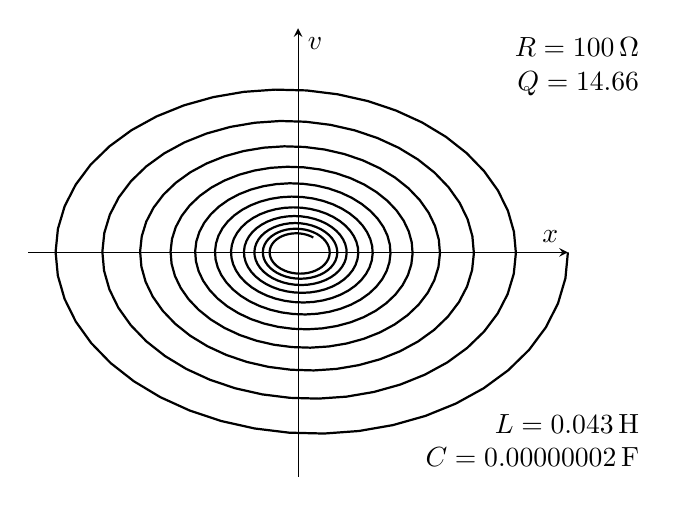
\begin{tikzpicture}[]
    \def\E{5}
    \def\R{100}
    \def\L{0.043}
    \def\C{0.00000002}
    \def\Q{(1/\R)*sqrt(\L/\C)}
    \def\wo{sqrt(1/(\L*\C))}
    \def\w{\wo*sqrt(1-1/(4*\Q^2))}
    % \def\Q{14.66}
    % \def\wo{34100}
    % \def\w{\wo*sqrt(1-1/(4*\Q^2))}
    \begin{axis}[
        xmin=-5, xmax=5,
        ymin=-0.004, ymax=0.004,
        xlabel=$x$, ylabel=$v$,
        axis lines=center,
        xtick=\empty, ytick=\empty,
        clip=false]
        \addplot[thick,
        domain=0:0.002,
        samples=500,
        black]
        ({\E*exp(-(\wo*\x)/(2*\Q))*(cos(\w*\x r)+(\wo/(2*\Q*\w))*sin(\w*\x r))},
        {\C*\E*exp(-(\wo*\x)/(2*\Q))*(-\w*sin(\w*\x r)*(1 + 1/(4*\Q^2-1)))});

        \node[anchor=north east, align=right] (RQtext) at (axis cs: 6.5, 0.004) {
                $R = \R\,\Omega$\\
                $Q = \fpeval{round(\Q,2)}$
        };
        \node[anchor=south east, align=right] (LCtext) at (axis cs: 6.5,-0.004) {
                $L = \L\,\rm H$\\
                $C = \C\,\rm F$
        };
    \end{axis}
\end{tikzpicture}
\end{document}
